\documentclass{article}
\usepackage[top=2cm, left=1.5cm, right=1.5cm, bottom=2cm]{geometry}
\usepackage{graphicx}
\usepackage{wrapfig}
\usepackage{amsmath}
\graphicspath{{./img/}}

\title{Systems of Linear Equations}
\date{16-Nov-2023}

\begin{document}
\maketitle
\section{What is a system of linear Equations?}

A linear equation in the variables $x_1,x_2,\dots, x_n $ is an equation that can be written in the form $ax_1,ax_2,\dots, ax_n = b$ where $b$ and the coefficients $ a_1, a_2,\dots, a_n $ an are real or complex numbers, the subscript $n$ may be any positive integer. In real-life problems, n might be 50 or 5000, or even larger. The equations \newline $$4x_1 - 5x_2 + 2 = x_1$$ $$x_2 = 2(\sqrt{6} - x_1) + x_3$$ \newline

Because they can be rearranged algebraically as:
$$3x_1-5_x2 = -2$$
$$2x_1 + x_2 - x_3 = 2 \sqrt{6}$$ 
The equations $$4x_1 - 5x_2 = x_1x_2$$ $$x_2 = 2\sqrt{x_1} - 6$$\newline are not linear because of the presence of $x_1, x_2$ in the first equation and $\sqrt{x1}$ in the second. A system of linear equations (or a linear system) is a collection of one or more linear equations involving the same variables. $$2x_1 - x_2 + 1.5x_3 = 8$$ $$x_1 \hspace{10 mm} - 4x_3 = -7$$\\
A solution of the system is a list $(s_1,s_2,\dots, s_n)$ of numbers that makes each equation a true statement when the values $(s_1,s_2,\dots, s_n)$ are substituted for $(x_1,x_2,\dots, x_n)$, respectively.
The set of all possible solutions is called the solution set of the linear system. Two linear systems are called equivalent if they have the same solution set.\newline

\subsection{Two Variables}

\begin{wrapfigure}{l}{0.3\textwidth} 
    \centering
    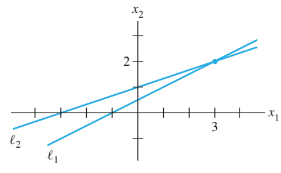
\includegraphics[width=0.3\textwidth]{image.png}
    \caption{1 Solution}
\end{wrapfigure}
Finding the solution set of a system of two linear equations in two variables is easy because it amounts to finding the intersection of two lines. Example: $$x_1 - 2x_2 = -1$$
$$-x_1 + 3x_2 = 3$$\newline
The graphs of these equations are lines, which we denote by $l_1$ and $l_2$. A pair of numbers $(x_1, x2_)$ satisfies both equations in the system if and only if the point $(x_1, x2_)$ lies on both $l_1$ and $l_2$. In the system above, the solution is the single point (3, 2).\pagebreak

\begin{wrapfigure}{r}{0.3\textwidth} 
    \centering
    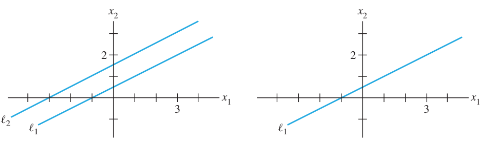
\includegraphics[width=0.3\textwidth]{image1.png}
    \caption{No solutions}
\end{wrapfigure}

Two lines need not intersect in a single point, they could be parallel, or they could coincide and hence “intersect” at every point on the line. For the graph 1, we dont have a solution, and for the graph 2, we have infinitely solutions. Thereforea system of linear equations has:

\begin{itemize}
    \item[-] No solution 
    \item[-] Exactly one solution
    \item[-] Infinitely many solutions \newline
\end{itemize} 

\noindent A system is said to be inconsistent if has no solution and a system is consistent if it has either 1 solution or infinitely solutions. If we are workin with 3 variables, we are looking a point that lies in the planes i.e.

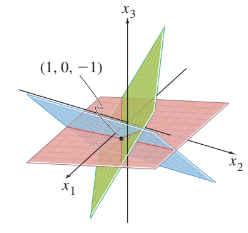
\includegraphics{image2.png}

In other dimensions we also have the same cases, there is no solution, there is one or infinite. In a third dimension the cases would look like this: 

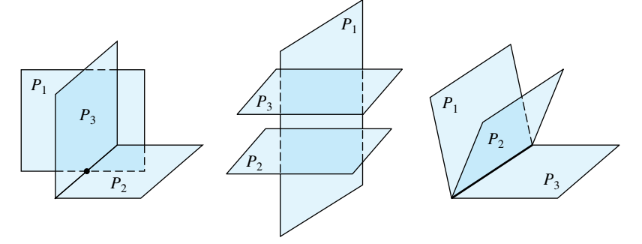
\includegraphics{image4.png}

\subsection{Matrix Notation}

The essential information of a linear system can be recorded compactly in a rectangular array called a matrix.

\begin{align*}
    \quad & x_1 - 2x_2 + \phantom{0} x_3 = 0 \\
    \quad & \phantom{1x_1+} 2x_2 -8x_3 = 8\\
    \quad & 5x_1 \phantom{+2x_2} -5x_3 = 10
\end{align*}

\pagebreak
Coefficient Matrix: the coefficients of each variable aligned in columns

$$\begin{bmatrix}
    1&-2&1\\
    0&2&-8\\
    5&0&-5
\end{bmatrix}$$

\noindent Augmented Matrix: coefficient matrix with an added column containing the constants from the right sides of the equation. \newline

$$\left[\begin{array}{ccc|c}
    1&-2&1&0 \\
    0&2&-8&8 \\
    5&0&-5&10 \pagebreak
\end{array}\right]$$

\subsection {Solving a Linear System}

The basic strategy is to replace one system with an equivalent system (one with the same solution set) that is easier to solve. Three elementary rows operations are used to simplify a linear system. 

\begin{itemize}
    \item[-] (Replacement) Replace one row by the sum of itself and a multiple of another row
    \item[-] (Interchange) Interchange two rows.
    \item[-] (Scaling) Multiply all entries in a row by a nonzero constant.
\end{itemize}

Example

\begin{equation}
    \begin{bmatrix}
        1 & -2 & 1 & 0\\
        0 & 2 & -8 & 8\\
        5 & 0 & -5 & 10
    \end{bmatrix}
\end{equation}

. \newline

Keep $x_1$ in the first equation and eliminate it from de other equations.

\begin{equation*}
    \begin{split}
        -5\cdot\text{[equation 1]}\\
        +\text{[equation 3]}\\
        \hline
        \text{[new equation 3]}
    \end{split}
\end{equation*}

Now in order to obtain 1 as the coefficient for $x_2$, multiply equation 2 by 1/2. With the 2 previous operations we obtain:

\begin{equation}
    \begin{bmatrix}
        1 & -2 & 1 & 0\\
        0 & 1 & -4 & 4\\
        0 & 10 & -10 & 10
    \end{bmatrix}
\end{equation}

Use $x_2$ in equation 2 to eliminate the $10x_2$ in equation 3.

\begin{equation*}
    \begin{split}
        -10\cdot\text{[equation 2]}\\
        +\text{[equation 3]}\\
        \hline
        \text{[new equation 3]}
    \end{split}
\end{equation*}

\begin{equation}
    \begin{bmatrix}
        1 & -2 & 1 & 0\\
        0 & 1 & -4 & 4\\
        0 & 0 & 30 & -30
    \end{bmatrix}
\end{equation}

Multiply equation 3 by 1/30 to obtain 1 as the coefficient for $x_3$:

\begin{equation}
    \begin{bmatrix}
        1 & -2 & 1 & 0\\
        0 & 1 & -4 & 4\\
        0 & 0 & 1 & -1
    \end{bmatrix}
\end{equation}

Use $x_3$ in equation 3 to eliminate the $-4x_3$ and $x_3$ in equations 1 and 2.

\begin{equation*}
    \begin{split}
        -1\cdot\text{[equation 3]}\\
        +\text{[equation 1]}\\
        \hline
        \text{[new equation 1]}
    \end{split}
\end{equation*}

\begin{equation*}
    \begin{split}
        4\cdot\text{[equation 3]}\\
        +\text{[equation 2]}\\
        \hline
        \text{[new equation 2]}
    \end{split}
\end{equation*}

\begin{equation}
    \begin{bmatrix}
        1 & -2 & 0 & 1\\
        0 & 1 & 0 & 0\\
        0 & 0 & 1 & -1
    \end{bmatrix}
\end{equation}

Finally move back to equation 2 and use it to eliminate the $-2x_2$ above it, since there is now no arithmetic involving $x_3$ terms.

\begin{equation*}
    \begin{split}
        \cdot\text{[equation 2]}\\
        +\text{[equation 1]}\\
        \hline
        \text{[new equation 1]}
    \end{split}
\end{equation*}

Obatining the final result:

\begin{equation}
    \begin{bmatrix}
        1 & 0 & 0 & \phantom{-}1\\
        0 & 1 & 0 & \phantom{-}0\\
        0 & 0 & 1 & -1
    \end{bmatrix}
\end{equation}

\begin{align*}
    \quad & x_1 \phantom{+x_2+x_3} = 1\\
    \quad & \phantom{x_1+} x_2 \phantom{+x_3} = 0\\
    \quad & \phantom{x_1+x_2+} x_3 = -1\\
\end{align*}

\begin{alignat*}{2}
    \begin{bmatrix}
       1 & 1 & 1 & 0 & 0 & 0\\
       0 & 0 & 0 & 1 & 1 & 1\\
       1 & 0 & 0 & 1 & 0 & 0\\
       0 & 1 & 0 & 0 & 1 & 0\\
       0 & 0 & 1 & 0 & 0 & 1\\
           \end{bmatrix}
        & \hspace{ 4em}%
      \begin{matrix} x_{11}x_{22}-x_{12}x_{21}=0 \\
      x_{11}x_{22}-x_{12}x_{21}=0 \\
      x_{11}x_{22}-x_{12}x_{21}=0 \\
     \end{matrix}
    \end{alignat*}
    \vskip1cm
    \begin{align*}
    \begin{bmatrix}
       1 & 1 & 1 & 0 & 0 & 0\\
       0 & 0 & 0 & 1 & 1 & 1\\
       1 & 0 & 0 & 1 & 0 & 0\\
       0 & 1 & 0 & 0 & 1 & 0\\
       0 & 0 & 1 & 0 & 0 & 1\\
           \end{bmatrix}
     \begin{bmatrix}
       x_{11} \\
       x_{12} \\
       x_{13} \\
       x_{21}\\
       x_{22}\\
       x_{23}\\
      \end{bmatrix}
        &=
    \begin{bmatrix}
       1 & 1 & 1 & 0 & 0 & 0\\
       0 & 0 & 0 & 1 & 1 & 1\\
       1 & 0 & 0 & 1 & 0 & 0\\
       0 & 1 & 0 & 0 & 1 & 0\\
       0 & 0 & 1 & 0 & 0 & 1\\
           \end{bmatrix}
     \begin{bmatrix}
       u_{11} \\
       u_{12} \\
       u_{13} \\
       u_{21}\\
       u_{22}\\
       u_{23}\\
      \end{bmatrix}%
       & \hspace{ 4em}%
      \begin{cases} x_{11}x_{22}-x_{12}x_{21}=0 \\
      x_{11}x_{22}-x_{12}x_{21}=0 \\
      x_{11}x_{22}-x_{12}x_{21}=0 \\
     \end{cases}\hspace{-1em}
    \end{align*}

It is important to note that row operations are reversible. Any solution of the original system remains a solution of the new system. Conversely, since the original system can be produced via row operations on the new system, each solution of the new system is also a solution of the original system.

\subsection{Existence and Uniqueness}

Is the system consistent; that is, does at least one solution exist?
If a solution exists, is it the only one; that is, is the solution unique?

Example : Determine if the following matrix is consistent: 

$\begin{matrix}
x_2 - 4x_3 = 8\\
2x_1 - 3x_2 + 2x_3 = 1\\
4x_1 - 8x_1 + 12x_3 = 1
\end{matrix}$

Converting the augmented matrix into the triangular form we obtain:

$\begin{matrix}
2x_1 - 3x_2 - 2x_3 = 1\\
x_2 - 4x_3 = 8\\
0 = 15
\end{matrix}$

The equation 3 is a short form of $0x_1 + 0x_2 + 0x_3 = 15$. This system has a built-in contradiction. There are no values of $x_1$, $x_2$, $x_3$ that satify because the equation $0=15$ is never true. Therefore the system is *inconsistent* (i.e. has no solution).

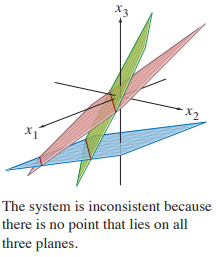
\includegraphics{image3.png}

\end{document}